\chapter{Implementação do Processo}
\label{chap:capacitor}
% ----------------------------------------------------------
A fim de confirmar as hipóteses de eficácia e eficiência do emprego do Processo
de Avaliação de Capacidade descrito no capítulo anterior, bem como da técnica de
Inferência de Desempenho e das Heurísticas de Seleção que dão suporte a esse Processo, 
criamos uma implementação concreta de sua especificação na forma de uma biblioteca
extensível e de um sistema computacional que demonstra seu funcionamento fazendo
a avaliação de uma aplicação real em um provedor de nuvem de infraestrutura.

Demos o nome de CloudCapacitor à biblioteca, implementada como uma \emph{gem} da
linguagem Ruby~\cite{ruby}. Desenvolvemos o sistema computacional Capacitor Web 
para ser uma interface visual para a utilização do CloudCapacitor, usando 
o \emph{framework} Ruby on Rails~\cite{rails}.  

Descrevemos a seguir os detalhes da implementação de cada um e como ambos se
relacionam para oferecer ao usuário a experiência da avaliação de capacidade
de baixo custo e alta precisão prevista pelo Processo proposto, com uma interface
amigável e de fácil utilização.

\section{CloudCapacitor}
CloudCapacitor é uma biblioteca para criação de sistemas de avaliação de 
capacidade em ambientes de nuvem de infraestrutura como serviço. É a implementação
completa da especificação do Processo de Avaliação de Capacidade do 
Capítulo~\ref{chap:processo}, permitindo que sejam customizadas as atividades 
definidas pelo Processo como pontos de extensão, como as Estratégias de Avaliação
e o disparo e controle da execução da Aplicação sob Teste.

Vamos iniciar a apresentação do CloudCapacitor pelas classes que compõem a biblioteca
e suas responsabilidades. Em seguida, veremos como CloudCapacitor auxilia 
desenvolvedores de software na criação de sistemas de avaliação de capacidade,
mostrando o fluxo de utilização da biblioteca através de sua interface de programação.
Depois, falaremos sobre alguns detalhes de implementação da biblioteca, como 
a solução para representação do Espaço de Implantação e seu papel na execução do
Processo de Avaliação de Capacidade. Por fim, apresentaremos os pontos de extensão
da biblioteca, notadamente como implementar um Executor, a classe responsável pelo
controle de execução da Aplicação sob Teste, e como sobrescrever a Estratégia de
Avaliação fornecida pela biblioteca a fim de alterar seu comportamento padrão.

Para concluir a apresentação do CloudCapacitor, será mostrada a saída de dados
fornecida pela biblioteca com as Configurações capazes de executar a
Aplicação sob Teste em cada uma das Cargas de Trabalho respeitando o SLA definido.

\subsection{Classes e Responsabilidades}
\label{subsec:classes}
CloudCapacitor é formado por um conjunto de classes que, juntas representam os
componentes envolvidos na avaliação de capacidade de aplicações em ambientes de
nuvem, de acordo com os conceitos e o Processo definidos anteriormente, nos
Capítulos~\ref{chap:formalizacao} e~\ref{chap:processo}. A Figura~\ref{fig:classes}
mostra as principais classes cujas responsabilidades e cooperação levam ao 
resultado final de uma Avaliação. 

Ao utilizar a biblioteca CloudCapacitor na construção de um software para avaliação
de capacidade, o desenvolvedor tem à sua disposição uma classe principal, chamada
\emph{Cacitor}. Essa classe fornece o fluxo principal do Processo de Avaliação, com todos
os seus pontos de decisão e de extensão.

\begin{figure}[htb]
  \caption{\label{fig:classes}Principais classes que compõem o CloudCapacitor e suas relações}
  \begin{center}
    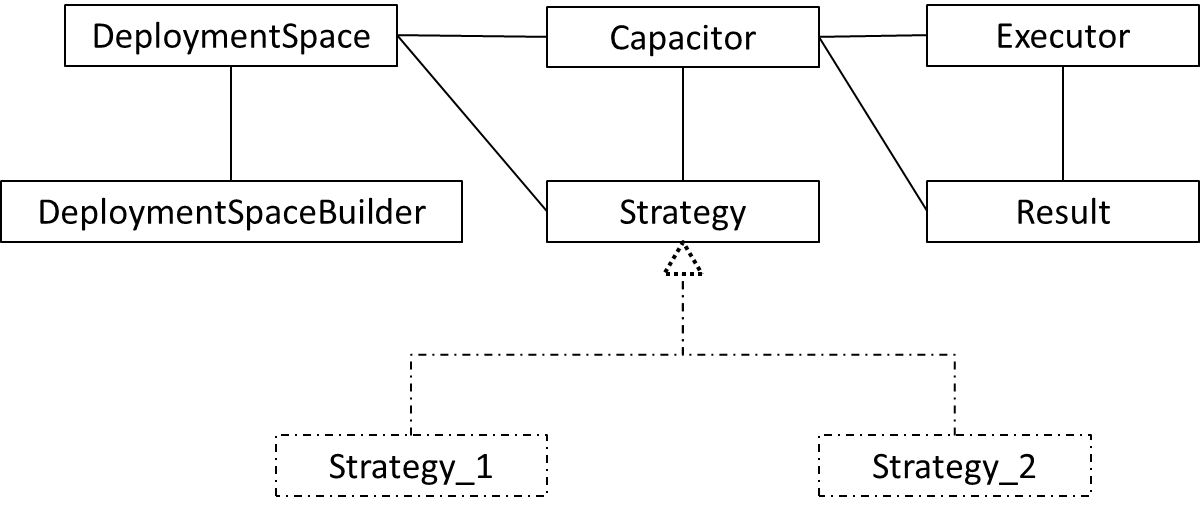
\includegraphics[scale=0.75]{img/CapacitorClasses}
  \end{center}
\end{figure}

Entre os pontos de extensão, destacamos o uso da classe \emph{Strategy}. Como 
vemos na Figura~\ref{fig:classes}, essa classe é fornecida pela biblioteca e a
notação de linhas pontilhadas denota a sua possibilidade de especialização, onde,
sobrescrevendo alguns de seus métodos, é possível criar Estratégias com comportamento
diversificado.

A classe \emph{DefaultExecutor} é o outro ponto de extensão oferecido pela biblioteca.
Porém, neste caso, o desenvolvedor deve mandatoriamente implementar uma subclasse
que forneça a lógica necessária ao controle da execução do teste de desempenho.
Na figura, a classe a ser implementada pelo desenvolvedor é representada com o 
nome de \emph{RealExecutor}.

Para que a Avaliação de Capacidade possa ser efetuada, a classe \emph{Capacitor}
deve conhecer o resultado de cada execução da Aplicação sob Teste, de modo que
possa tomar as decisões corretas na indicação das Configurações Candidatas e
Rejeitadas. Esses resultados são encapsulados na classe \emph{Result}, cujos 
objetos são fornecidos pela subclasse responsável pela execução dos testes de 
desempenho.

E, finalmente, durante a execução da Avaliação de Capacidade, a classe \emph{Capacitor} 
precisa ter conhecimento do Espaço de Implantação disponibilizado. Essa é a 
responsabilidade da classe \emph{DeploymentSpace}, que implementa uma estrutura 
de dados em memória para representar os diversos Níveis de Capacidade formados 
entre as Configurações. A construção dessa estrutura é responsabilidade da classe 
\emph{DeploymentSpaceBuilder}, que contém os algoritmos necessários à preparação 
do grafo usado para navegação pelos Níveis de Capacidade. 

\subsection{Fluxo de Utilização da Biblioteca}
\label{subsec:fluxo}
CloudCapacitor foi criada para ser uma ferramenta de auxílio na construção de 
aplicações destinadas à condução de testes para avaliação de capacidade,
visando basicamente a reusabilidade e a simplicidade na composição dessas 
aplicações.

Embora tenha sido desenvolvida objetivando sua utilização na construção de 
aplicações web baseadas no framework Ruby on Rails, CloudCapacitor pode facilmente
ser usada em todo tipo de aplicação escrita em Ruby, desde scripts puros até
aplicações baseadas em outros frameworks.

Em suma, o fluxo de utilização da biblioteca é bastante simples e pode ser 
descrito por:

\begin{enumerate}
  \item Configurar parâmetros de criação do Espaço de Implantação 
  \item Identificar Tipos de Máquinas Virtuais para o Espaço de Implantação
  \item Instanciar um objeto \emph{Capacitor}
  \item Atribuir ao \emph{Capacitor} um objeto \emph{DefaultExecutor}
  \item Atribuir ao \emph{Capacitor} um objeto \emph{Strategy}
  \item Executar o método \emph{run\_for} do \emph{Capacitor}
\end{enumerate}

Antes que a aplicação que está sendo desenvolvida possa de fato dar início ao uso 
da biblioteca, é preciso que o desenvolvedor a configure previamente. 

O primeiro passo é configurar os limites de tamanho do Espaço de Implantação e 
isso deve ser feito através de um arquivo em formato YAML~\cite{yml}. A localização 
e o nome do arquivo de parâmetros para a criação do Espaço de Implantação dependem 
de como a aplicação está sendo implementada: se for uma aplicação Ruby on Rails, 
deverá haver um arquivo chamado \emph{capacitor.yml} na pasta \emph{config}, que 
fica dentro da pasta raiz da aplicação; caso contrário, deverá haver um arquivo 
chamado \emph{capacitor\_settings.yml} já na pasta raiz da aplicação ou na mesma 
pasta em que está o script que invoca a biblioteca. 

A Figura~\ref{fig:settings} mostra um exemplo de conteúdo do arquivo que configura
os limites do Espaço de Implantação. São apenas dois parâmetros:

\begin{description}
  \item[max\_price] \hfill \\ O custo máximo que uma Configuração pode atingir
  \item[max\_num\_instances] \hfill \\ Número máximo de instâncias usadas em uma Configuração 
\end{description}

\begin{figure}[h]
  \caption{\label{fig:settings}Parâmetros de Configuração para o CloudCapacitor}
 \begin{lstlisting}[linewidth=\textwidth,xleftmargin=.04\textwidth, numbers=left]
deployment_space:
  #The maximum price for a whole Configuration.
  #This refers to the individual VM_Type price multiplied 
  #by the number of instances that make up the Configuration
  max_price: 7.0

  #The maximum number of instances in a Configuration. 
  #This is for horizontal scaling.
  max_num_instances: 4
  \end{lstlisting}
\end{figure}

No exemplo acima, serão criadas Configurações com 1, 2, 3 e 4 instâncias para cada
Tipo de Máquina Virtual especificada, desde que o custo total da Configuração não
ultrapasse o valor de 7,00 unidades monetárias.

O próximo passo na utilização do CloudCapacitor é especificar quais serão os Tipos
de Máquinas Virtuais utilizados na geração do Espaço de Implantação. Essa 
especificação é feita em outro arquivo em formato YAML, discriminando as 
características de CPU, Memória e custo de cada Tipo de Máquina para que o
CloudCapacitor possa gerar os Níveis de Capacidade usados para inferência de
desempenho. O caminho onde esse arquivo deve ser entrado precisa ser passado 
como parâmetro na inicialização do objeto Capacitor. Caso não seja informado, o 
CloudCapacitor procurará um arquivo pelo nome \emph{deployment\_space.yml}, na
pasta \emph{config}, se for uma aplicação Ruby on Rails, ou na pasta raiz do
script ou outro tipo de aplicação.
 
\begin{figure}[h]
  \caption{\label{fig:depspace}Especificação de Tipos de Máquinas para o Espaço de Implantação}
 \begin{lstlisting}[linewidth=\textwidth,xleftmargin=.04\textwidth, numbers=left]
---
- !ruby/object:CloudCapacitor::VMType
  name: m2.xlarge
  cpu: 6.5
  mem: 17.1
  price: 0.41
  category: m2
- !ruby/object:CloudCapacitor::VMType
  name: c1.xlarge
  cpu: 20
  mem: 7.0
  price: 0.58
  category: c1
- !ruby/object:CloudCapacitor::VMType
  name: m1.xlarge
  cpu: 8
  mem: 15.0
  price: 0.48
  category: m1
- !ruby/object:CloudCapacitor::VMType
  name: m2.4xlarge
  cpu: 26
  mem: 68.4
  price: 1.64
  category: m2
  \end{lstlisting}
\end{figure}

A Figura~\ref{fig:depspace} mostra a especificação de um conjunto de Tipos de
Máquinas Virtuais oferecidos pelo serviço EC2 do Provedor Amazon Web 
Services~\cite{ec2}. São disponibilizadas para o CloudCapacitor máquinas 
\emph{m2.xlarge}, \emph{c1.xlarge}, \emph{m1.xlarge} e \emph{m2.4xlarge} e, para
cada uma, podemos ver as características de CPU, memória RAM e preço, conforme
informados pelo Provedor. Esses são os dados que serão usados na criação do Espaço
de Implantação, atendendo às restrições de tamanho e custo impostas no passo 
anterior, de forma que os testes sejam executados conforme o proposto
no Processo de Avaliação de Capacidade.

Feitas as configurações necessárias, o desenvolvedor pode, assim, criar um objeto 
a partir da classe \emph{Capacitor} e, então atribuir a ele um objeto instanciado
a partir de uma subclasse de \emph{DefaultExecutor}, subclasse esta de sua própria
implementação e que forneça os meios necessários para administração da execução
dos testes de desempenho da Aplicação sob Teste.

\begin{figure}[h]
  \caption{\label{fig:mincode}Código Ruby para execução do CloudCapacitor}
 \begin{lstlisting}[language=Ruby,linewidth=\textwidth,xleftmargin=.04\textwidth, numbers=left]
    capacitor = Capacitor.new
    capacitor.executor = Executors::DummyExecutor.new
    capacitor.strategy = Strategies::Strategy.new

    capacitor.strategy.approach workload: :optimistic,
                                config:   :conservative

    candidates = capacitor.run_for [100,200,300,400,500]
    
    total_cost = capacitor.run_cost
    total_executions = capacitor.executions  
 \end{lstlisting}
\end{figure}

Observamos na Figura~\ref{fig:mincode} os passos de instanciação do Capacitor,
na linha 1. Na linha seguinte, um objeto da classe \emph{DummyExecutor}, que é
apenas didática, já é atribuído ao \emph{Capacitor}.

A partir da linha 3, começamos a ver os passos seguintes da utilização do 
CloudCapacitor, com a definição de uma Estratégia de Avaliação, configurada
com uma Heurística de Seleção do tipo OC (v. Seção~\ref{sec:heuristicas}).
A execução da Avaliação de Capacidade acontece de fato na chamada que ocorre
na linha 8, onde são passados valores que representam uma lista de grandezas de
Cargas de Trabalho que serão impostas à Aplicação sob Teste rodando sobre as
Configurações geradas a partir do Espaço de Implantação.

Ao final da Avaliação, o Capacitor retorna a lista de Configurações Candidatas
para cada valor de Carga de Trabalho passado como parâmetro. Adicionalmente, o
desenvolvedor tem à sua disposição alguns dados a respeito da própria Avaliação,
como o número total de execuções da Aplicação sob Teste no ambiente de nuvem e o  
custo total acarretado por essas execuções. 

Agora que já temos uma visão geral dos componente e da utilização do CloudCapacitor,
passemos a uma descrição um pouco mais detalhada do que acontece durante a atividade
de Avaliação de Capacidade.

\subsection{Funcionamento Interno}
\label{subsec:capacitor_funcionamento}
Uma vez demonstrado o modelo de utilização da biblioteca e explicadas as relações
entre as diversas classes que a compõem, podemos detalhar alguns aspectos da
implementação que ajudarão a esclarecer melhor como todas essas partes agem em
conjunto para executar, da forma como proposto no Capítulo~\ref{chap:processo},
o Processo de Avaliação de Capacidade.

Nesta seção mostraremos inicialmente as linhas gerais da implementação da classe 
responsável pelo controle da execução dos testes de desempenho. Mostraremos em 
seguida como a biblioteca representa o Espaço de Implantação de forma que os 
Níveis de Capacidade sejam usados para navegar entre Configurações e como a 
Inferência de Desempenho atua sobre esses dados. Explicamos ainda como pode ser 
feita a customização de uma Estratégia de Avaliação a fim de alterar o 
comportamento de uma Heurística. Será também apresentado um exemplo de saída do 
resultado apresentado pela classe Capacitor ao final da execução de uma Avaliação.

\subsubsection{Controle da Execução}
\label{subsubsec:funcionamento_executor}
O controle da execução da Aplicação sob Teste no ambiente de nuvem é feito por 
meio de um objeto instanciado de uma classe que deve ser criada pelo
desenvolvedor que está utilizando o CloudCapacitor na implementação de sua 
ferramenta de Avaliação de Capacidade.

Para que tudo funcione a contento, a classe criada deve ser extendida a partir
da classe \emph{DefaultExecutor} fornecida pelo CloudCapacitor. A única 
exigência feita para essa subclasse é que ela implemente um método:

\begin{itemize}
  \item Com a assinatura \emph{run(configuration, workload)}; e
  \item Que retorne um objeto da classe \emph{Result}
\end{itemize}

Ou seja, a classe criada pelo desenvolvedor deve pelo menos apresentar um método
\emph{run} que receba como parâmetros uma Configuração e um valor para a Carga 
de Trabalho que será imposta sobre a Aplicação. O retorno desse método deve ser
um objeto da classe \emph{Result}, que deve ser inicializado com apenas 3 atributos:

\begin{description}
  \item[\emph{value}] \hfill \\
    O valor obtido pela Aplicação para a Métrica de Desempenho estudada
  \item[\emph{cpu}] \hfill \\
    O percentual de CPU consumido pela Aplicação durante o teste
  \item[\emph{mem}] \hfill \\
    O percentual de Memória RAM utilizada pela Aplicação durante o teste
\end{description}

Essas informações devem ser obtidas pelo desenvolvedor através de chamadas a
uma ferramenta de execução de testes, como \cite{cunha2012ambiente}, 
\cite{jayasinghe2012} ou \cite{silva2013cloudbench}. A implementação dessa 
comunicação com a ferramenta de automação de testes escolhida é efetuada está 
fora do escopo deste trabalho e deve ficar a cargo do desenvolvedor prover o 
código que controle a execução dos testes e obtenha os valores de desempenho
e consumo de CPU e memória.

O método \emph{run}, implementado na subclasse criada a partir de 
\emph{DefaultExecutor}, é chamado pelo objeto \emph{Capacitor} nos momentos em
que novas execuções são necessárias, conforme descrito na 
Seção~\ref{subsec:processo_execucao}. O objeto \emph{Result} retornado é usado
na comparação com o SLA especificado pelo usuário do sistema como Valor de
Referência para indicar se a Aplicação atendeu ou não ao requisito de desempenho.

De posse dessa resposta, o \emph{Capacitor} tem condições de prosseguir no seu
processamento, marcando as Configurações como Candidatas ou Rejeitadas e 
escolhendo as próximas Configurações a serem executadas. Essas ações se baseiam
no caminhamento sobre o Espaço de Implantação, cuja implementação passamos a
descrever a seguir.

\subsubsection{Espaço de Implantação}
\label{subsubsec:funcionamento_depspace}
O uso do CloudCapacitor começa com as configurações de como a 
biblioteca vai montar o Espaço de Implantação, apontando-se quais as restrições 
e quais os Tipos de Máquinas disponíveis para realização dos testes.

No momento em que o desenvolvedor instancia um objeto da classe \emph{Capacitor},
uma das primeiras tarefas da biblioteca é exatamente proceder à montagem de uma
estrutura que represente o Espaço de Implantação de forma que as Heurísticas
possam navegar entre as Configurações e que a rotina que implementa o Processo de
Avaliação possa identificar, por meio da técnica de Inferência de Desempenho, 
quais são as Configurações Candidatas e Rejeitadas. 

\begin{figure}[htb]
  \caption{\label{fig:depspace_real}Representação interna de um Espaço de Implantação no CloudCapacitor}
  \begin{center}
    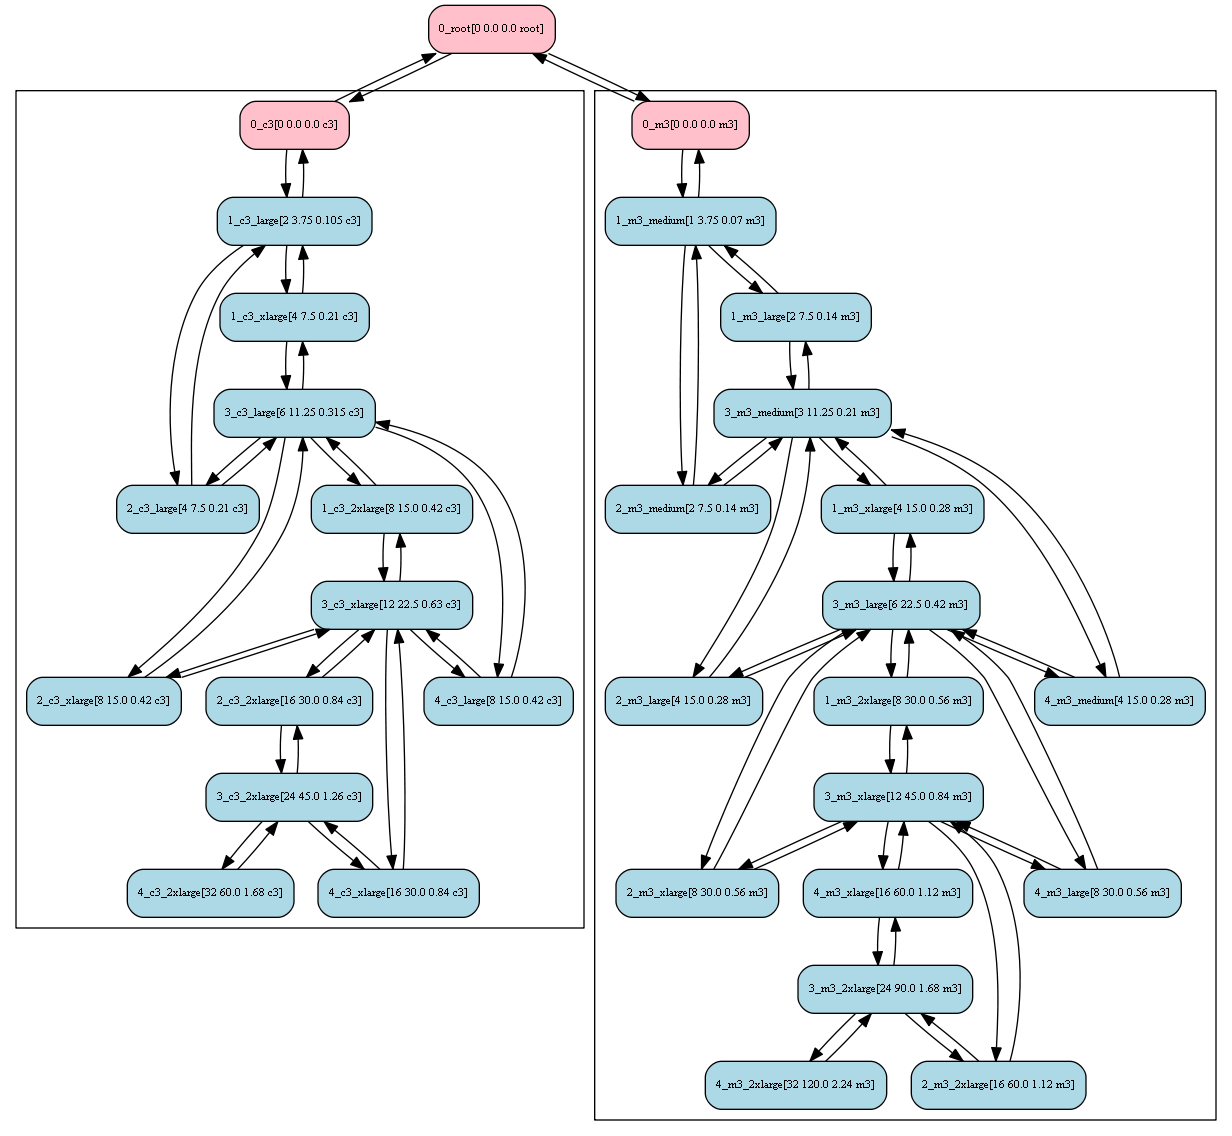
\includegraphics[scale=0.35]{img/exemplo_grafo_espaco_implantacao}
  \end{center}
\end{figure}

Como é possível ver na Figura~\ref{fig:depspace_real}, o Espaço de Implantação é 
representado internamente por um grafo bi-direcionado onde os nós são as 
Configurações. Arestas existem entre nós onde sejam verdadeiras as relações 
``maior que'' e ``menor que'', conforme as definições da 
Seção~\ref{sec:formalizacao_configuracoes}. O grafo precisa ser bi-direcionado 
para permitir que a navegação a partir de uma determinada Configuração seja feita 
tanto para as Configurações ``maiores'' quanto para as ``menores''.

CloudCapacitor separa o Espaço de Implantação em subgrafos, agrupando as
Configurações por Categoria de Máquinas Virtuais. Cada subgrafo é destinado às
Configurações cujo Tipo de Máquina pertença a uma determinada Categoria. O primeiro
nó, observado no topo do grafo, é o nó raiz e serve apenas para estabelecer a 
separação e permitir o trânsito entre as Categorias.

As classes \emph{DeploymentSpace} e \emph{DeploymentSpaceBuilder} implementam
a geração do Espaço de Implantação com base na relação de capacidade ou na relação
de preço entre as Configurações. O desenvolvedor pode optar pelo grafo por capacidade ou por preço no momento da
instanciação do objeto \emph{Capacitor}. Embora esse não seja o foco desta 
pesquisa, isso foi feito para que pudesse ser estudada a influência da formação 
do Espaço de Implantação na precisão e eficiência de custo das Heurísticas de 
Seleção. Discutiremos a respeito desses resultados no Capítulo~\ref{chap:resultados} 
adiante.

O Espaço de Implantação é a estrutura que dá suporte à navegação das Estratégias
sobre os diversos Níveis de Capacidade no momento em que devem ser escolhidas
as próximas Configurações a serem testadas. Suporta também a técnica de Inferência 
de Desempenho na identificação das relações de tamanho e/ou preço entre as 
Configurações nos pontos onde o Processo marca as Candidatas ou Rejeitadas, 
mostrando-se como um ponto chave para o sucesso do Processo de Avaliação.

Descreveremos a seguir a implementação e o funcionamento das Estratégias de 
Avaliação e como o desenvolvedor pode criar sua própria Estratégia que melhor
supra suas necessidades de seleção de Configurações. 

\subsubsection{Estratégias de Avaliação}
\label{subsubsec:funcionamento_estrategias}
A Estratégia de Avaliação é responsável por aplicar uma Heurística de 
Seleção de Configurações nos momentos em que o Processo precisa navegar
pelo Espaço de Implantação. Assim, a cada momento em que um novo Nível 
de Capacidade deve ser escolhido, segundo o fluxo de ações previsto no 
Processo de Avaliação proposto, a Estratégia é invocada e age conforme 
a implementação da Heurística selecionada para a Avaliação.

CloudCapacitor fornece uma classe chamada \emph{Strategy} como uma implementação
padrão para as 9 Heurísticas descritas no Capítulo~\ref{chap:processo}. A
Figuras~\ref{fig:strategy_workload_code}~e~\ref{fig:strategy_capacity_code}
mostram o código fonte dos métodos de seleção de Carga de Trabalho e Nível
de Capacidade, respectivamente.

\begin{figure}[h]
  \caption{\label{fig:strategy_workload_code}Seleção de Carga de Trabalho na classe \emph{Strategy}}
  \begin{lstlisting}[language=Ruby,linewidth=\textwidth,xleftmargin=.04\textwidth, numbers=left]
  def select_workload( workload_list )
    case @wkl_approach
      when :pessimistic
        workload_list.first
      when :optimistic
        workload_list.last
      when :conservative
        workload_list[ workload_list.size / 2 ]
    end
  end
  \end{lstlisting}
\end{figure}

\begin{figure}[h]
  \caption{\label{fig:strategy_capacity_code}Seleção de Nível de Capacidade na classe \emph{Strategy}}
  \begin{lstlisting}[language=Ruby,linewidth=\textwidth,xleftmargin=.04\textwidth, numbers=left]
  def take_a_capacity_level_from( unexplored_levels )
    levels = unexplored_levels.keys
    return [] if levels.empty?
    case @cfg_approach
      when :pessimistic
        unexplored_levels.assoc( levels[-1] )
      when :optimistic
        unexplored_levels.assoc( levels[0] )
      when :conservative
        unexplored_levels.assoc( levels[levels.size / 2] )
    end
  end
  \end{lstlisting}
\end{figure}

Porém,
é possível substituir essa classe por uma mais adequada aos objetivos do
usuário.

A interface da classe \emph{Capacitor} permite que 

Figura~\ref{fig:mincode}

***RASCUNHO***
CloudCapacitor
OK  Diagrama de Classes (UML) / Arquitetura de Componentes
OK  Enumeração das classes e suas responsabilidades
OK  Fluxo de utilização da biblioteca (caixa preta, interface com o Capacitor)
OK  Especificação e Carregamento do Deployment Space
  Executor - Implementação
  Estratégia - Descrição da interface
  Estratégia - Como sobrescrever (Gof Strategy Pattern)
  Apresentação do resultado da avaliacao
Capacitor Web
  Apresentação da interface de entrada
  Resultados
  Trace
  Full Trace
Resumo e transicao para o proximo capitulo
***RASCUNHO***



PorémAo instanciar um objeto da classe Capacitor, o desenvolvedor deve atribuir  
Por padrão, o CloudCapacitor oferece uma Estratégia de Avaliação que implementa 
uma lógica simples para as Heurísticas de Seleção de Configurações definidas no
capítulo anterior. Essa lógica pode ser facilmente sobrescrita conforme a necessidade
do usuário ou o perfil da Aplicação sob Teste.


****RASCUNHO
\subsection{Heuristicas}
Para que uma Heurística de Avaliação de Capacidade seja compatível no âmbito deste trabalho, 
deve apresentar um conjunto mínimo de operações esperadas para que a lógica da
avaliação se complete e o resultado final obtido possa ser considerado válido e
comparável com os resultados obtidos por outras Heurísticas.

Além disso, as operações constituem a interface pela qual o controlador das 
sessões de avaliação pode configurar as Heurísticas e informar-lhe os dados 
necessários ao controle da sua execução.
 
Apresentamos esse conjunto mínimo de operações nas subseções a seguir, que 
representam o arcabouço necessário para a construção de uma Heurística de 
Avaliação de Capacidade.
 
% ----------------------------------------------------------
